\documentclass[11pt,a4paper,ngerman]{article}
\usepackage[bottom=2.5cm,top=2.5cm]{geometry} 
\usepackage{babel}
\usepackage[utf8]{inputenc} 
\usepackage[T1]{fontenc} 
\usepackage{ae} 
\usepackage{amssymb} 
\usepackage{amsmath}
\usepackage{amsthm} 
\usepackage{graphicx}
\usepackage{fancyhdr}
\usepackage{fancyref}
\usepackage{listings}
\usepackage{xcolor}
\usepackage{paralist}

\usepackage[pdftex, bookmarks=false, pdfstartview={FitH}, linkbordercolor=white]{hyperref}
\usepackage{fancyhdr}
\pagestyle{fancy}
\fancyhead[C]{Advanced Functional Programming}
\fancyhead[L]{Exercise sheet 2}
\fancyhead[R]{SoSe 2013}
\fancyfoot{}
\fancyfoot[L]{}
\fancyfoot[C]{\thepage \hspace{1px} of \pageref{LastPage}}
\renewcommand{\footrulewidth}{0.5pt}
\renewcommand{\headrulewidth}{0.5pt}
\setlength{\parindent}{0pt} 
\setlength{\headheight}{0pt}

\date{}
\title{Exercise sheet 2}
\author{Max Wisniewski, Alexander Steen}


%%
%% Enviroments for proofs and lemmas
%%
\newtheorem{lemma}{\bfseries lemma}
\newtheorem{claim}{\bfseries claim}

\lstloadlanguages{Haskell}
\lstset{
  language=Haskell,
  basicstyle=\ttfamily,
  flexiblecolumns=false,
  basewidth={0.5em,0.45em},
  literate={+}{{$+$}}1 {/}{{$/$}}1 {*}{{$*$}}1 {=}{{$=$}}1
           {>}{{$>$}}1 {<}{{$<$}}1 {\\}{{$\lambda$}}1
           {\\\\}{{\char`\\\char`\\}}1
           {->}{{$\rightarrow$}}2 {>=}{{$\geq$}}2 {<-}{{$\leftarrow$}}2
           {<=}{{$\leq$}}2 {=>}{{$\Rightarrow$}}2 
           {\ .}{{$\circ$}}2 {\ .\ }{{$\circ$}}2
           {>>}{{>>}}2 {>>=}{{>>=}}2
           {|}{{$\mid$}}1               
}

\lstnewenvironment{code}
    {\lstset{basicstyle=\footnotesize\ttfamily}%
      \csname lst@SetFirstLabel\endcsname}
    {\csname lst@SaveFirstLabel\endcsname}
\long\def\ignore#1{}

\begin{document}

\renewcommand{\figurename}{Figure}
\maketitle
\thispagestyle{fancy}

\section*{Task 1}
We first prove a lemma that is being used in the induction proof of the task's proposition:
\textbf{Lemma}: \lstinline|f (foldNat' f e n) = foldNat' f (f e) n|.\\
\textbf{Proof} by induction:\\
Base: \texttt{n = O}
    \begin{lstlisting}
      f (foldNat' f e O)
    = {Def.}
      f e
    = {Def. inverse}
      foldNat' f (f e) O
    \end{lstlisting}
Step: \texttt{n} $\rightsquigarrow$ \texttt{S n}
    \begin{lstlisting}
      f (foldNat' f e (S n))
    = {Def.}
      f (foldNat' f (f e) n)
    = {Induction Hyp.}
      foldNat' f (f (f e)) n
    = {Def. inverse}
      foldNat' f (f e) (S n)
    \end{lstlisting}
\mbox{} \hfill $\square$

\textbf{Proposition}: \lstinline|foldNat f e = foldNat' f e|.\\
\textbf{Proof} by induction:\\
Base: \texttt{n = O}
    \begin{lstlisting}
      foldNat f e O
    = {Def.}
      e
    = {Def. inverse}
      foldNat' f e 0
    \end{lstlisting}
Step: \texttt{n} $\rightsquigarrow$ \texttt{S n}
    \begin{lstlisting}
      foldNat f e (S n)
    = {Def.}
      f (foldNat f e n)
    = {Induction Hyp.}
      f (foldNat' f e n)
    = {Lemma}
      foldNat' f (f e) n
    = {Def. inverse}
      foldNat' f e (S n)
    \end{lstlisting} 
\mbox{} \hfill $\square$
\documentclass[11pt,a4paper,ngerman]{article}
\usepackage[bottom=2.5cm,top=2.5cm]{geometry}
\usepackage[ngerman]{babel}
\usepackage[utf8]{inputenc}
\usepackage[T1]{fontenc}
\usepackage{ae}
\usepackage{amssymb}
\usepackage{amsmath}
\usepackage{amsthm}
\usepackage{graphicx}
\usepackage{fancyhdr}
\usepackage{fancyref}
\usepackage{listings}
\usepackage{xcolor}
\usepackage{stmaryrd}
\usepackage{paralist}
\usepackage{tikz}
\usepackage{amsthm}

\usetikzlibrary{arrows,automata}

\newtheorem{propo}{Satz}
\newtheorem{lemmas}[propo]{Lemma}

\usepackage[pdftex, bookmarks=false, pdfstartview={FitH}, linkbordercolor=white]{hyperref}
\usepackage{fancyhdr}
\pagestyle{fancy}
\fancyhead[C]{ADS}
\fancyhead[L]{Übung 2}
\fancyhead[R]{SoSe 2014}
\fancyfoot{}
\fancyfoot[L]{}
\fancyfoot[C]{\thepage \hspace{1px} of \pageref{LastPage}}
\renewcommand{\footrulewidth}{0.5pt}
\renewcommand{\headrulewidth}{0.5pt}
\newcommand{\set}[1]{ \{ #1 \}}
\setlength{\parindent}{0pt}
\setlength{\headheight}{0pt}

\newcommand{\N}{\mathbb{N}}
\newcommand{\Q}{\mathbb{Q}}
\newcommand{\R}{\mathbb{R}}
\newcommand{\bigO}{\mathcal{O}}
\newcommand{\Rarr}{\Rightarrow}
\newcommand{\rarr}{\rightarrow}
\newcommand{\Pot}{\mathcal{P}}
\newcommand{\abs}[1]{\left |#1\right|}
\newcommand{\solved}{$\mbox{}$ \hfill $\square$}
\newcommand{\Epsilon}{\mathcal{E}}

\newcommand{\erw}[1]{\text{\bfseries E} \left[ #1 \right]}
\newcommand{\prob}[1]{\text{Pr}\left[ #1 \right]}

\date{}
\title{Übung 2}
\author{Max Wisniewski, Melanie Skodzik}


%%
%% Enviroments for proofs and lemmas
%%
\newtheorem{prop}{\bfseries Behauptung}
\newtheorem{lemma}{\bfseries Lemma}

\begin{document}

\lstset{language=Pascal, basicstyle=\ttfamily\fontsize{10pt}{10pt}\selectfont\upshape, commentstyle=\rmfamily\slshape, keywordstyle=\rmfamily\bfseries, breaklines=true, frame=single, xleftmargin=3mm, xrightmargin=3mm, tabsize=2, mathescape=true}

\renewcommand{\figurename}{Figure}

\maketitle
\thispagestyle{fancy}


\subsection*{Aufgabe 1}

Eine plausible Alternative zu Splay-Bäumen besteht darin, die Operationen \emph{splay(x)} durch eine Operation \emph{moveToRoot(x)} zu ersetzen, welche den Knoten $x$ durch wiederholte Links- bzw. Rechtsrotationen n die Wurzel befürdert. Der resultierende Algortihmus wird als \emph{MTR-Heuristik} bezeichnet.

Wie unterscheidet sich die MTR-Heuristik von Splay-Bäumen? Zeigen Sie durch eine explizite Konstruktion, dass die MTR-Heuristik im worst-case amortiesierte Laufzeit $\Omega(n)$ ausfweisen kann. Dabei ist $n$ die Anzahl der Elemente im Suchbaum.\\

\noindent\textbf{Beweis:}\\

Die MTR-Heuristik unterscheidet sich vom Splay-Baum nur in einer einzelnen Situation, nämlich im zick-zick-Schritt. Im zick-zack- und im zick-Schritt ist die splay Operation nämlich auch einfach eine eine Rotation um den nach oben zu bewegenden Knoten. Der zick-zick Schritt bei Splay-Bäumen rotiert aber einmal um den Großvater(-mutter) von $x$ und nicht direkt um $x$.\\

Damit wir also eine andere Laufzeit als bei Splay-Bäumen erhalten, muss unser Worst-Case möglichst viele zick-zick-Schritte benötigen -- oder einen Baum, der bei Splay-Bäumen einen zick-zick-Schritt auslöst. Dazu beweisen wir den folgenden Satz.\\

Wir betrachten nur Suchoperationen.

\begin{propo}\label{ads:ueb2:mtrheu} (Worstcase Folgen Laufzeit)
   Sei $T$ ein binärer Suchbaum mit Knoten $\{1, \ldots, n\}$ 
   ein listenförmiger Baum mit nur linken Kindern. 

   \begin{center}
   \begin{tikzpicture}[font=\small, minimum size=0.5cm]
      \node[draw=black,name=a] {$n$};
      \node[draw=black, name=b, below left of=a] {$n-1$};
      \node[name=c, below left of =b] {$\ldots$};
      \node[draw=black, name=d, below left of = c] {$2$};
      \node[draw=black, name=e, below left of =d] {$1$};

      \path[-]
         (a) edge (b)
         (b) edge (c)
         (c) edge (d)
         (d) edge (e);
   \end{tikzpicture}
   \end{center}

   Dann 
   ist die Laufzeit der Anfragefolge $A = a_1, \ldots, a_n$ mit 
   $a_i = i$ $\Theta(n^2)$ und der Baum sieht nach $A$ aus wie zu Beginn.
\end{propo}

Für diesen Satz führen wir zunächst zwei Hilfssaätze ein.

\begin{lemmas} \label{ads:ueb2:lemma1} (Ankerlemma)\\
   Wird \emph{moveToRoot} auf den minimalen Knoten $1$ in der Kette wie in Satz \ref{ads:ueb2:mtrheu} auf gerufen, resultiert dies in einem Baum

   \begin{center}
   \begin{tikzpicture}
      \node[draw=black,name=a] {$1$};
      \node[draw=black, name=b, below right of=a] {$n$};
      \node[name=c, below left of =b] {$\ldots$};
      \node[ draw=black, name=d, below left of = c] {$2$};

      \path[-]
         (a) edge (b)
         (b) edge (c)
         (c) edge (d);
   \end{tikzpicture}
   \end{center}

   Die Laufzeit hierbei beträgt $\Theta(n^2)$.
\end{lemmas}

\begin{lemmas} \label{ads:ueb2:lemma2} (Schrittlemma)\\
   Wenden wir moveToRoot auf $l_1$ im linken Baum an, so erhalten wir den rechten Baum. 

   \begin{center}
      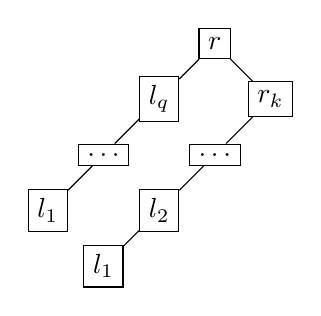
\begin{tikzpicture}
         \node[draw=black,name=root] {$r$};
         \node[draw=black,name=lt, below left of = root] {$l_q$};
         \node[draw=black,name=lm, below left of = lt] {$\ldots$};
         \node[draw=black,name=lb, below left of = lm] {$l_1$};
         \node[draw=black,name=rt, below right of = root] {$r_k$};
         \node[draw=black,name=rm, below left of = rt] {$\ldots$};
         \node[draw=black,name=rb1, below left of = rm] {$l_2$};
         \node[draw=black,name=rb2, below left of = rb1] {$l_1$};

         \path[-]
            (root) edge (lt)
                   edge (rt)
            (lt)  edge  (lm)
            (lm)  edge  (lb)
            (rt)  edge  (rm)
            (rm)  edge  (rb1)
            (rb1) edge  (rb2);
      \end{tikzpicture}
      $\;\leadsto\;$
      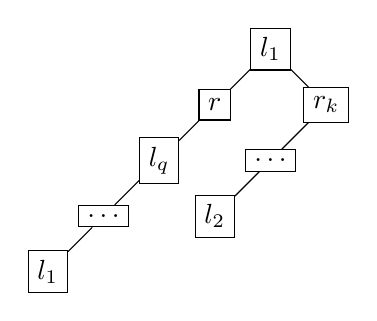
\begin{tikzpicture}
         \node[draw=black,name=rb2] {$l_1$};
         \node[draw=black,name=root,below left of = rb2] {$r$};
         \node[draw=black,name=lt, below left of = root] {$l_q$};
         \node[draw=black,name=lm, below left of = lt] {$\ldots$};
         \node[draw=black,name=lb, below left of = lm] {$l_1$};
         \node[draw=black,name=rt, below right of = rb2] {$r_k$};
         \node[draw=black,name=rm, below left of = rt] {$\ldots$};
         \node[draw=black,name=rb1, below left of = rm] {$l_2$};

         \path[-]
            (rb2) edge  (root)
                  edge  (rt)
            (root) edge (lt)
            (lt)  edge  (lm)
            (lm)  edge  (lb)
            (rt)  edge  (rm)
            (rm)  edge  (rb1);
      \end{tikzpicture}
   \end{center}

   Dabei beträgt die Laufzeit genau $\Theta(k+1)$.
\end{lemmas}

Beweisen wir zunächst die beiden Lemmas.\\

\noindent\textbf{Beweis \ref{ads:ueb2:lemma1}.}\\
Wir machen eine Induktion über $n$. Die Anker sind trivial, da bei $n=1$ nichts passiert und $n=2$ genau die Definition der Linksrotation ist.
Betrachtet werden muss also nur noch der Induktionsschritt.\\

Wir haben also unsere Kette von $1$ bis $n+1$. Führen wir nun moveToRoot durch, wird erst die Kette von $1$ bis $n$ durchgegangen und hochrotiert.
Dies führt nach I.V. zu einer Kette der Form 

   \begin{center}
   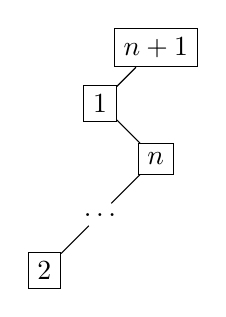
\begin{tikzpicture}
      \node[draw=black,name=root] {$n+1$};
      \node[draw=black,name=a, below left of = root] {$1$};
      \node[draw=black, name=b, below right of=a] {$n$};
      \node[name=c, below left of =b] {$\ldots$};
      \node[ draw=black, name=d, below left of = c] {$2$};

      \path[-]
         (root) edge (a)
         (a) edge (b)
         (b) edge (c)
         (c) edge (d);
   \end{tikzpicture}
   \end{center}

Führen wir rauf noch eine Rotation auf $1$ aus, so erhalten wir noch Definition der Rotation den gewünschten Baum.

Haben wir nun für den Baum der Höhe $n$ genau $c \ cdot n$ Rotationen gebraucht, so benötigen wir nun $c \cdot (n+1)$ Rotationen und die Laufzeit ergibt sich.

\mbox{}\hfill$\square$

\noindent\textbf{Beweis \ref{ads:ueb2:lemma2}.}\\
Wir machen eine Induktion über $k$. Die Anker sind wir in Lemma \ref{ads:ueb2:lemma1} trivial, da es genau der Definition der Rotation entspricht. Im Schritt
nehmen wir die Kette der Länge $k+1$. Für die Kette von $r_1 \ldots r_k$ können wir Lemma \ref{ads:ueb2:lemma1} benutzen.
 
      \begin{center}  
     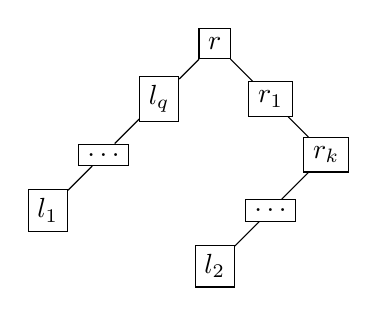
\begin{tikzpicture}
         \node[draw=black,name=root] {$r$};
         \node[draw=black,name=lt, below left of = root] {$l_q$};
         \node[draw=black,name=lm, below left of = lt] {$\ldots$};
         \node[draw=black,name=lb, below left of = lm] {$l_1$};
         \node[draw=black,name=rt, below right of = root] {$r_1$};
         \node[draw=black,name=rt2, below right of = rt] {$r_k$};
         \node[draw=black,name=rm, below left of = rt2] {$\ldots$};
         \node[draw=black,name=rb1, below left of = rm] {$l_2$};

         \path[-]
            (root) edge (lt)
                   edge (rt)
            (lt)  edge  (lm)
            (lm)  edge  (lb)
            (rt)  edge  (rt2)
            (rt2)  edge  (rm)
            (rm)  edge  (rb1);
      \end{tikzpicture}
      \end{center} 
Nun können wir $r_1$ in einer Rotation auf die andere Seite bringen und haben den Zielbaum erreicht. Wir benätigen wiederum eine Rotation mehr als die Kette mit $k+1$ Elementen. Daher kommen wir insgesammt auf eine Laufzeit von $\Theta(k)$.

\mbox{}\hfill$\square$

Mit diesen beiden wenden wir uns dem Satz zu.

\noindent\textbf{Beweis \ref{ads:ueb2:mtrheu}.}
Wir zeigen, dass nach $j$ Schritten der Baum aussieht, wie in Lemma \ref{ads:ueb2:lemma2} mit einer Kette rechten Kette der Länge $n-j$ und einer linken Kette
der Länge $j-1$, wobei das $j$-te Element die Wurzel ist.
\begin{description}
   \item[\bfseries Anker:] Wenden wir auf die Kette der Länge $n$ die erste Operation $a_1 = 1$ an, so erhalten wir als Ergebnis einfach
         Lemma \ref{ads:ueb2:lemma1}. Die rechte Kette ist um $1$ kürzer, die Linke ist noch $0$ lang und $1$ ist die Wurzel.
   \item[\bfseries Schritt:] $j \rightarrow j+1$\\
         Wenden wir auf die Kette der Länge $n$ die I.V. an, so erhalten wir die Vorraussetzung für Lemma \ref{ads:ueb:lemma2}
         mit einer rechten Kette der Länge $n-j$ einer linken Kette der Länge $j-1$ und als Wurzel $j$. Rufen wir nun moveToRoot auf $j+1$ auf,
         so erhalten wir nach Lemma \ref{ads:ueb:lemma2} einen Baum mit einer Linken Kette von Länge $j$ einer Wurzel von $j+1$ und die rechte Kette ist auch
         um eins Kürzer.
\end{description}
Nach der $n$-ten Operation ist die rechte Kette $0$ lang und wir haben nur eine linke Kette mit $n$ Elementen, wenn wir die Wurzel dazu zählen. Da Rotationen
die Sortierung aufrecht erhalten gibt es mit den Elementen $\{1, \ldots , n\}$ nur einen einzigen Baum, der so aussieht und dies ist der Startbaum.

Die Laufzeit für eine solche Kette von $n$ Operationen beträgt
$$
   T(n) = n + \sum_{i=1}^n i = n + \frac{n*(n-1)}{2} = \Theta(n^2).
$$
\mbox{}\hfill$\square$

Nun müssen wir diesen Satz nur noch nehmen und auf beliebige Ketten von $n$ erweitern.

\begin{propo} \label{ads:ueb2:mtrheuend}
   Für einen links-kettenförmigen binären Suchbaum $T$ mit Elemente $\{1, \ldots, n\}$ hat die Folge
   $A = a_1, \ldots, a_m$ mit $a_i = (i \text{ mod } n) + 1$ die Laufzeit $\Theta(m \cdot n)$.

   Damit ist die amortisierte Laufzeit für eine einzelne Operation $\Omega(n)$.
\end{propo}

\noindent\textbf{Beweis \ref{ads:ueb2:mtrheuend}.}\\
   Wir haben hier $m \text{ div } n$ mal die Operationskette aus Satz \ref{ads:ueb2:mtrheu}. Die Vorraussetzungen sind wie gezeigt nach jedem mal wieder hergestellt.
   Wir müssen also nur noch beweisen, dass der letzte angebrochene Versuch nicht die Laufzeit kaputt macht.

   $$\begin{array}{rcl}
      T(n) = (m \text{ div } n) \sum_{i=1}^n i + 2 \cdot n + (m \text{ mod } n) \sum_{i=n}^{m \text{ mod } n} i\\
           = (\left\lceil \frac{m}{n} \right\rceil) \cdot \frac{n(n+1}{2} - \sum_{i=1}^{m \text{ mod } n}
           = \Theta (m \cdot n)
   \end{array}$$
   Im falle, dass wir im linken Teil zu viel nehmen und auf $+1$ kommen ziehen wir im rechten Teil nicht ganz so viel ab, wie der Faktor im linken Teil ist,
   wir bewegen uns also zwischen $m \cdot n$ und $(m+1) \cdot n$. Dies liegt eindeutig in $\Theta(m\cdot n)$.\\

   Für die amortiesierten Kosten müssen wir die Gesammtkosten durch die Anzahl der Operationen teilen. Wir erhalten so also $\Theta(n)$ und somit auch $\Omega(n)$.

   \mbox{}\hfill$\square$








\subsection*{Aufgabe 2}

\subsubsection*{(a)}
Beweisen Sie : Seien $a,b > 0$ und $c \geq a+ b$. Dann ist
$$
   \log \, a + \log \, b \leq 2 \log \, c - 2.
$$

\noindent\textbf{Beweis:}\\
Seien $a,b,c$ wie im Satz.\\

Wir beweisen zunächst eine etwas schwächere Aussage.
$$\begin{array}{crcl}
   & \log \, a + \log \,b &=& 2 \log \, (a+b) - 2\\
\Leftrightarrow & \log \, (a\cdot b) &\leq & \log \, \frac{(a+b)^2}{4}\\
\Leftrightarrow & 4ab & \leq & (a+b)^2\\
\Leftrightarrow & 4ab & \leq & a^2 + 2ab + b^2\\
\Leftrightarrow & 0 & \leq & a^2 - 2ab + b^2\\
\Leftrightarrow & 0 & \leq & (a-b)^2
\end{array}$$
Gilt trivialer weise, da das quadrat einer rationalen Zahl immer größer oder gleich $0$ ist.

Nun folgt aus der monotonie des Logarithmus, dass für $c \geq a+b$
$$
   \log \, (a+b) \leq \log \, c
$$
Und somit die gesammte Aussage.

\mbox{}\hfill$\square$

\subsubsection*{(b)}

Nehmen Sie an, ein Splaybaum enthält die Elemente $1, \ldots, n$ und bearbeitet eine Folge $A = a_1, \ldots a_n$ von $m$ Suchanfragen mit $a_i\in\{1,\ldots,n\}$. Beweisen Sie den Satz vom \emph{statischen Finger}.\\

Sei $f\in\{1,\ldots,n\}$ fest. Dann ist die Gesammtlaufzeit für die Folge $A$
$$
   O(n \log \, n + m + \sum_{i=1}^m \log \, (|a_i - f| + 1)).
$$

\noindent\textbf{Beweis:}\\

tbd

\subsection*{Aufgabe 3}
Benutzen Sie den Codierungssatz von Shannon um die folgende Aussage zu beweisen.

Sei $T$ ein fester binärer Suchbaum, der die Elemente $\{1,\ldots,n\}$ enthält und sei $A=a_1,\ldots,a_m$ eine Folge von $m$ Suchanfragen, die jedes Element mindestens einmal enthält. Sei $q_i$ die Anzahl der Anfragen an das Element $i$. Dann ist die Gesammlaufzeit für $A$ mindestens
$$
   \Omega\left(m + \sum_{i=1}^n q_i \log \frac{m}{q_i}\right)
$$

\noindent\textbf{Beweis:}\\

tbd



\label{LastPage}
\end{document}


\label{LastPage}

\end{document}
